
\documentclass[
12pt, % Main document font size
a4paper, % Paper type, use 'letterpaper' for US Letter paper
oneside, % One page layout (no page indentation)
%twoside, % Two page layout (page indentation for binding and different headers)
%headinclude,footinclude, % Extra spacing for the header and footer
%BCOR5mm, % Binding correction
]{article}


%	Text
\usepackage[utf8]{inputenc}		% <-- Darstellung von Umlauten
\usepackage[T1]{fontenc}
\usepackage[ngerman]{babel}
%\usepackage[toc,page]{appendix} % Appendix

\usepackage{multicol} %Mehrere Spalten


% Filter out unwanted warnings and error messages
\usepackage{silence}
  \WarningFilter{latex}{Marginpar}


%	Tabellen
\usepackage{booktabs} % Better horizontal rules in tables
\usepackage{units} % Used for printing standard units

%	Grafiken
\usepackage{graphicx} % Needed to insert images into the document
\graphicspath{{graphics/}} % Sets the default location of pictures
\setkeys{Gin}{width=\linewidth,totalheight=\textheight,keepaspectratio} % Improves figure scaling
\usepackage{epstopdf} % Einbinden von EPS
\usepackage{tikz}

% Bibtex
\usepackage{natbib}

% Listen 
\usepackage{enumitem}

% Header
\usepackage{fancyhdr}
\pagestyle{fancy}
%%%% ---> Start HEADER

%\rhead{\includegraphics[width=1cm]{DLR_Signet_schwarz.jpg}}
%\lhead{Tap3D}
\setlength\headheight{28pt} 

%%%%% <----- End Header

\hyphenation{Fortran hy-phen-ation} % Specify custom hyphenation points in words with dashes where you would like hyphenation to occur, or alternatively, don't put any dashes in a word to stop hyphenation altogether

%----------------------------------------------------------------------------------------
%	TITLE AND AUTHOR(S)
%----------------------------------------------------------------------------------------


%\title{%
%  Vorhabensbeschreibung \\
%  \large Zur Bekanntmachung
%Innovation durch Additive Fertigung
%}
%\author{M.S.} % The article author(s) - author affiliations need to be specified in the AUTHOR AFFILIATIONS block
%\date{\today} % An optional date to appear under the author(s)

%----------------------------------------------------------------------------------------

\begin{document}

\setlength\parindent{0pt} % Kein Einzug nach Absatz


%\maketitle % Print the title/author/date block

\begin{titlepage}
	\centering
	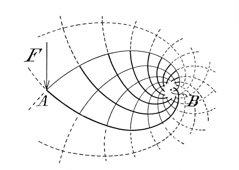
\includegraphics[width=0.5\textwidth]{michell_cantilever.jpg}\par\vspace{1cm}
	{\scshape\LARGE Literaturübersicht \par}
	\vspace{0.5cm}
	{ über den Themenbereich \par}
	\vspace{1.5cm}
	{\huge\bfseries Topologie Optimierung\par}
	%\vspace{0.3cm}
	%{Verbindung aus \textbf{Tap}elege und  \textbf{3D}-Druck Prozess für die Fertigung hochintegrierter Leichtbaustrukturen\par}
	\vspace{7cm}
	{Deutsches Zentrum für Luft und Raumfahrt (DLR) \par}
	{Institut für Bauweisen und Strukturtechnologie \par}
	\vspace{0.3cm}
	{Pfaffenwaldring 30-40 \par}
	{70569 Stuttgart \par}

	%{\Large\itshape John Birdwatch\par}
	%\vfill
	%supervised by\par
	%Dr.~Mark \textsc{Brown}

	\vfill

% Bottom of the page
	%{\large \today\par}
\end{titlepage}



%\setcounter{tocdepth}{2} % Set the depth of the table of contents to show sections and subsections only
%\tableofcontents % Print the table of contents
%\listoffigures % Print the list of figures
%\listoftables % Print the list of tables





\section{Literatur Übersicht} % (fold)
\label{sec:literaturueberblick}



% section literaturueberblick (end)

\newpage


sdfsdf
\newpage
\newpage
\bibliographystyle{plain}
\bibliography{LieraturAdd}
%\bibliographystyle{plainnat} % Use the plainnat style of referencing

\end{document}{}